\documentclass[12pt]{article}
\usepackage{amsfonts,amsmath,amssymb, listings}

\usepackage[utf8]{inputenc}
\usepackage{graphicx}
\usepackage{multirow}
\usepackage{xcolor}

\usepackage{threeparttable}
\usepackage{blindtext}


\usepackage[a4paper, total={6in, 8in}]{geometry}

\usepackage[numbered,framed]{matlab-prettifier}
%\usepackage{color}

%\setcounter{MaxMatrixCols}{10}

\def\stackunder#1#2{\mathrel{\mathop{#2}\limits_{#1}}}%

\newcommand{\fiid}{\func{i.i.d.}} % use this as in: X_i \stackrel{\fiid}{\sim} \func{Exp} \left( \lambda \right)
\DeclareMathOperator{\Norm}{N}

\newcommand{\platzo}{\vspace*{2cm}}
\newcommand{\platzt}{\vspace*{4cm}}

\newcommand{\findep}{\func{ind}}  % could use indep instead if ind, but 1st book uses ind.

\newcommand{\R}{\ensuremath{{\mathbb R}}}
\newcommand{\N}{\ensuremath{{\mathbb N}}}
\def\QATOP#1#2{{#1 \atop #2}}
\def\QTATOP#1#2{{\textstyle {#1 \atop #2}}}
\def\QDATOP#1#2{{\displaystyle {#1 \atop #2}}}
\voffset=-2.54cm\hoffset=-2.54cm \textheight27cm \textwidth17.0cm \topmargin0.5cm
\oddsidemargin2.00cm \evensidemargin2.00cm \unitlength1cm

\def\func#1{\mathop{\rm #1}}%
\def\dint{\mathop{\displaystyle \int}}%
\newcommand{\Ind}{\ensuremath{{\mathbb I}}} % indicator function
\newcommand{\E}{\ensuremath{{\mathbb E}}} % expected value
\newcommand{\Var}{\ensuremath{{\mathbb V}}} % variance

\setlength{\parindent}{0pt}

\usepackage{float}

\newfloat{Program}{thp}{lop}[section]
\floatname{Program}{Program Listing}

\begin{document}

\pagestyle{empty}

\bigskip

\begin{figure}[htp]
    \centering
    
\includegraphics[width=4cm]{uzh logo 2.png}
    \label{fig:UZH}
\end{figure}

\begin{Large}
	\begin{center}
		\textbf{Digital Tools for Finance}
	\end{center}
\end{Large}

\vspace{2cm}

\begin{large}	
	\begin{center}
		\textbf{Effect of Interest Rate Changes on Cryptocurrencies} \vspace{0.1cm} \\ {Prof. Igor Pozdeev } \vspace{2cm} \\ \textbf{Matthias Olieslagers - 22714034}  \\ \textbf{
Cameron Storey - 22740815} \\
        \textbf{Marc David Parker - 22727762}\\
        \textbf{Qian Chen - 21742226}\\
	\end{center}
\end{large}

\tableofcontents

\newpage

\bigskip
\section{Introduction}

The goal of this research report is to discover how changes in FED interest rates have an impact on the prices of cryptocurrencies (e.g. Bitcoin) \newline
In the first section, the different data sources will be covered. What does the data exactly represent and why is it relevant to look into for this particular research. In the second part, the methodology will be laid out. Lastly, the results will be critically evaluated and interpreted and a final conclusion will be provided. 
\newline Before we dive in, let's give some introduction on the FED rate and what our initial hypothesis of this research will be. \newline 

The Federal Reserve, or FED, is the central banking system of the United States. One of its main responsibilities is setting interest rates, which can have a significant impact on the overall economy. 

To understand the potential relationship between the FED rate and Bitcoin price, it is first necessary to understand the role that interest rates play in the economy. When the FED raises interest rates, it becomes more expensive for businesses and individuals to borrow money. This can have a dampening effect on economic activity, as people and companies are less likely to take out loans for things like purchasing homes, cars, or investing in new businesses. On the other hand, when the FED lowers interest rates, it becomes cheaper to borrow money, which can encourage increased spending and investment.

Given this, it is logical to assume that changes in the FED rate could potentially affect the price of Bitcoin. If the FED raises interest rates, for example, it could potentially lead to a decrease in demand for risky assets like Bitcoin, as investors may be more hesitant to take on additional risk when borrowing costs are higher. On the other hand, if the FED lowers interest rates, it could potentially lead to an increase in demand for risky assets like Bitcoin, as investors may be more willing to take on additional risk when borrowing costs are lower.
\newline
It is thus unclear upfront to predict which force of these two will have most effect on the actual Bitcoin price and whether or not there will be other main macro economic factors that play an important role, which makes this research question all the more interesting. 
\section{Data}

The datasets that were used to develop an answer to this research question are the BTC-USD Daily Price and the FED rate, both over the extensive time period from 2016 to date. At first, we also looked at several other currencies such as Solana and the Dogecoin, but decided not to include them in the final analysis as their values are less representative for the market. We also looked at other interest rate metrics, such as the LIBOR and SOFR rate. These two interest rates relatively close follow the path of the FED rate and they are both continuous rates. All of the data was obtained from reliable sources such as Yahoo Finance and MarketWatch.



\section{Analysis}
\subsection{Methodology}
In this paragraph, we will dig deeper on the methodology for the analysis and explain and interpret the results. The extensive explanation (e.g. all of the underlying code, plots etc.) can be found in the Jupyter notebook, this report serves as a brief summary of the main findings. \newline \newline
The programming language Python, with extensions pandas, numpy and matplotlib, is used and the following approach is used. First, we read in the BTC and FED data and some of the functions for the calculation of metrics such as the Moving Average and Rolling Volatily are defined. These metrics will be used in the analysis later on. Next, the particular dates at which there was effectively a change in the FED rate are highlighted and sorted out, we will obviously focus on these particular dates when assessing what the effect of an interest change on the crypto prices is. \newline
\newline As an illustration, the graph below (see Figure \ref{fig:FED Rate evolution 2016 - 2022}) illustrates the evolution of the FED rate across the last 6 years. As can be seen, this is a stepwise function, so there are no daily changes but rather periodical changes with flat periods in between. \newline It is interesting to note that the macro-economic events can clearly be seen in the graph. At the beginning of 2020, the interest rate drops to a low point in order to support the economy during the Covid-19 outbreak. Now since the beginning of 2022, the interest rate has started to rise sharply in order to slow down the inflation. The FED rate is thus a tool to regulate the economy and in the next paragraph down below we will discuss whether these changes have any significant impact on the prices of BTC.

\begin{figure}[!htb]
   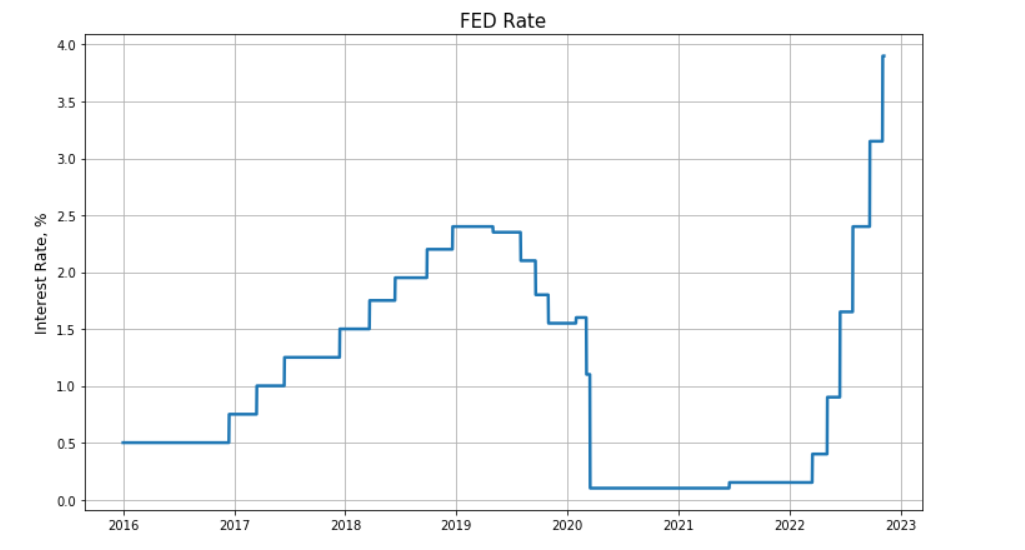
\includegraphics[scale=0.6]{research_project/text/paper/FED rate graph.png}
   \centering
   \caption{FED Rate evolution 2016 - 2022}
   \label{fig:FED Rate evolution 2016 - 2022}
\end{figure}


\subsection{Price fluctuations}
First we looked at the FED rate changes and if there is an n-day correlation after these changes had taken place for n=1,2,...,8. The change is recorded from the close, the day before the FED rate change.
\begin{center}
\begin{tabular}{|l|l|l|l|l|l|l|l|l|}
\hline
Change & 1 Day  & 2 Day  & 3 Day  & 4 Day & 5 Day  & 6 Day  & 7 Day  & 8 Day  \\ \hline
FED    & -0.122 & -0.072 & -0.138 & -0.22 & -0.157 & -0.197 & -0.273 & -0.242 \\ \hline
\end{tabular}
\end{center}
From this we see that there is no significant relationship between a certain day after the change takes place and a movement in BTC price movements.\\
\newline
\subsection{Moving Averages}
Next we decided to investigate if the change in FED rate had any directional impact on the value for the moving average over serval periods.
\begin{figure}[H]
   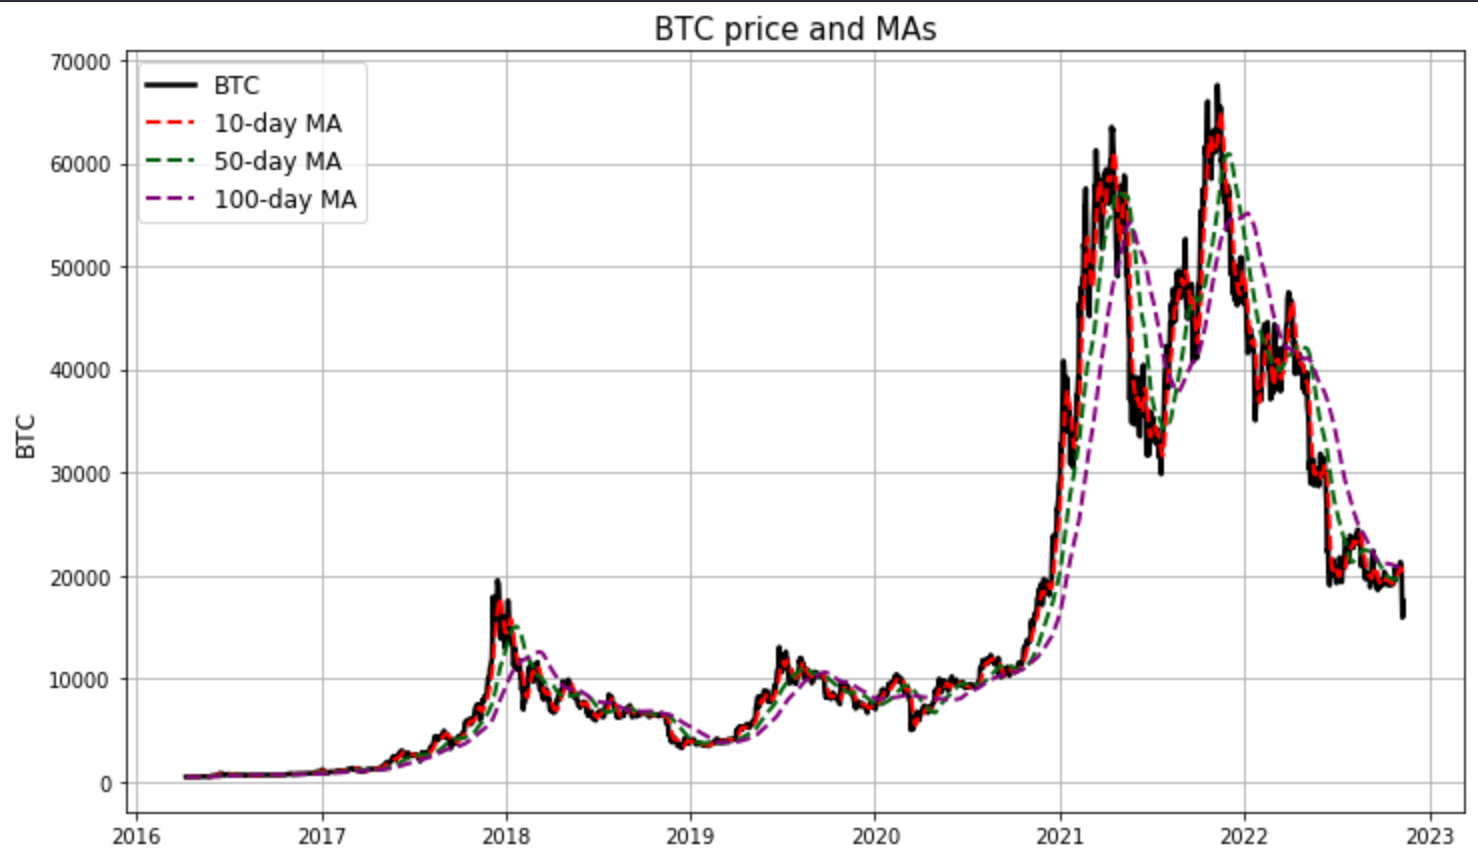
\includegraphics[scale=0.6]{research_project/text/paper/2.png}
   \centering
   \caption{Moving averages against price}
   \label{fig:ma}
\end{figure}
We checked whether the change in moving average after an announcement was "out of the ordinary". To do it, we first find  95\% confidence intervals for MA with different time span (where we choose 10, 50 and 100 days). Then we check whether the MA where the FED rate changes behaves some ``abnormality". By ``abnormality" we mean the MA data is not inside the according confidence interval. In every case, we found that the MA value after a FED rate change lies within this interval.
\begin{figure}[H]
   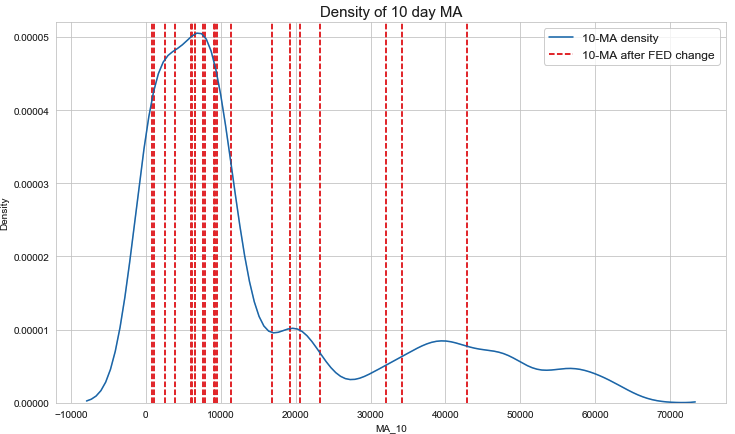
\includegraphics[width=\textwidth]{research_project/text/paper/density10ma.png}
   \centering
   \caption{Density of 10-day MA and the FED changing dates }
   \label{fig:10dayma}
\end{figure}
We can see in the above plot, the distribution of the 10-day moving average values and the values after (in red) a FED rate change. We see clearly that these values are not our of the ordinary and would lead us to believe there is not directional relationship between BTC and the FED rate. 
\subsection{Volatility Analysis}
Because we observed no significant finding from the analysis in the previous section we have decided to analyse if the changes in FED rate make any difference on the volatility of BTC price.\\
Below is an example of the 20 day rolling volatility of BTC.
\begin{figure}[H]
   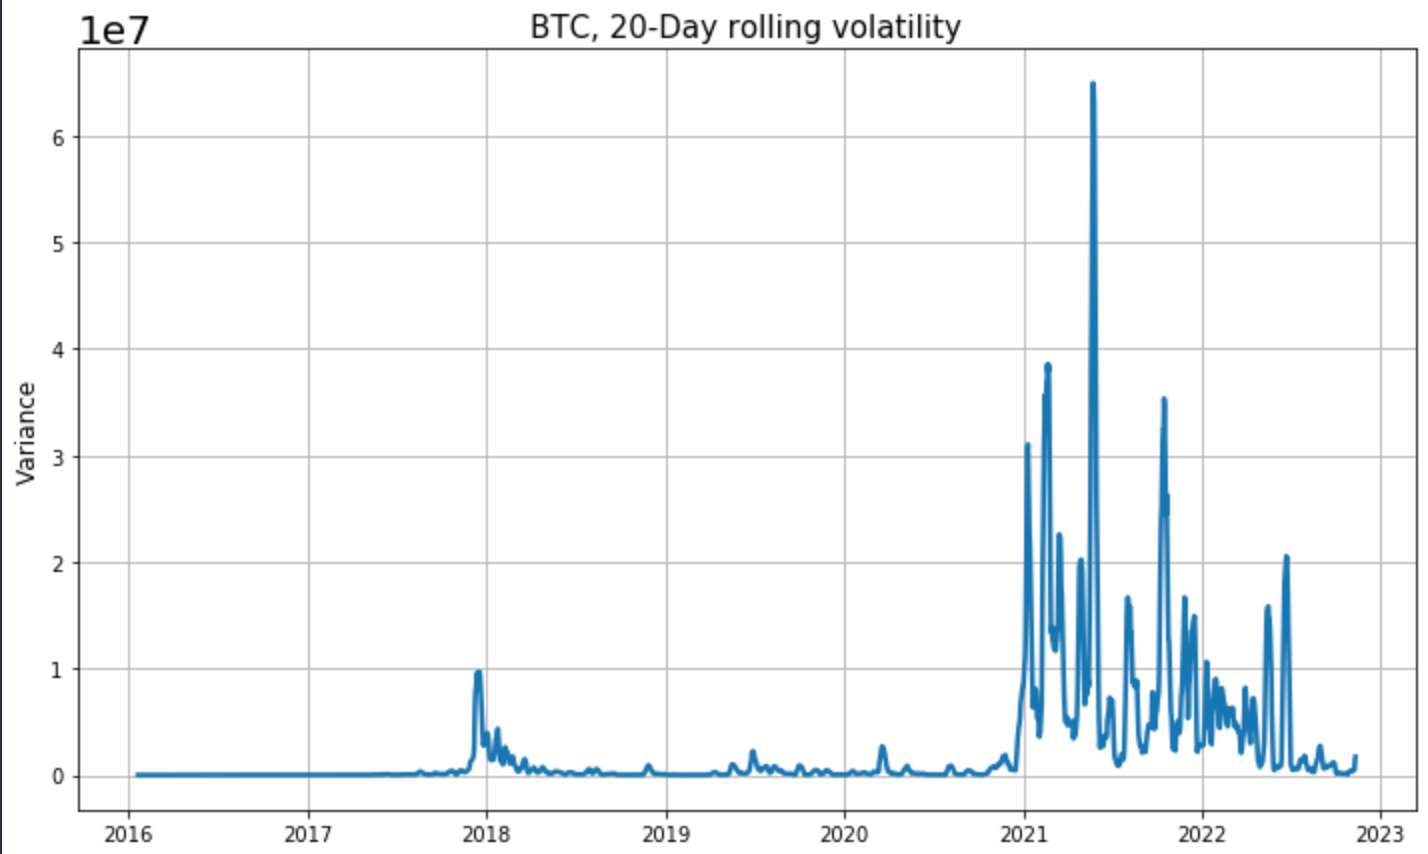
\includegraphics[scale=0.6]{research_project/text/paper/6.png}
   \centering
   \caption{BTC volatility}
   \label{fig:FED Rate evolution 2016 - 2022}
\end{figure}

As we increase the period, the graph becomes smoother.
\newline
Performing a similar analysis as we did for the moving averages. We can see in the figure below that the observed volatility after a FED rate change was not abnormal for what has been observed over the course of the data.
\begin{figure}[H]
   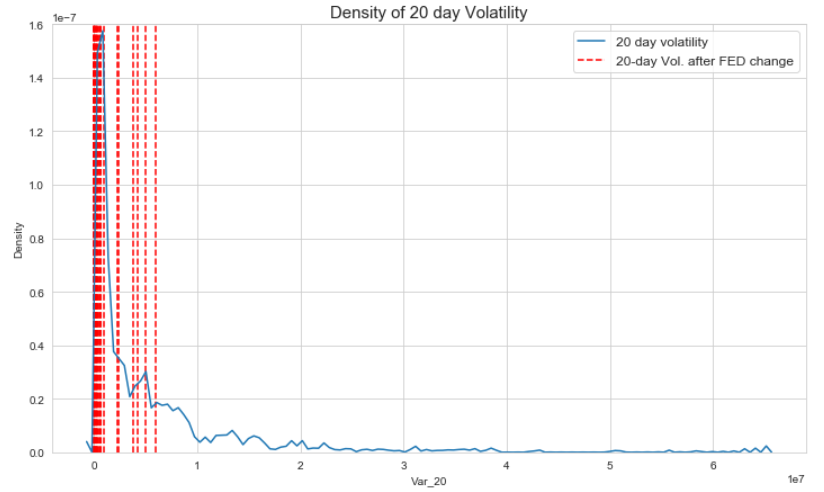
\includegraphics[scale=0.6]{research_project/text/paper/image1.png}
   \centering
   \caption{Density of 20-day rolling vol. and the FED changing dates }
   \label{fig:rolling_vol20}
\end{figure}
We did this for periods 5,10 and 20 days and saw no significant results.
\subsection{Daily Range}
Another metric we have decided to look at was the daily change, the daily high minus the daily low of the day, this is another metric for volatility but will be more sensitive day-to-day. 
\newline
In the figure below, we can see how the BTC daily range evolves respective to the FED rate change.
\begin{figure}[H]
   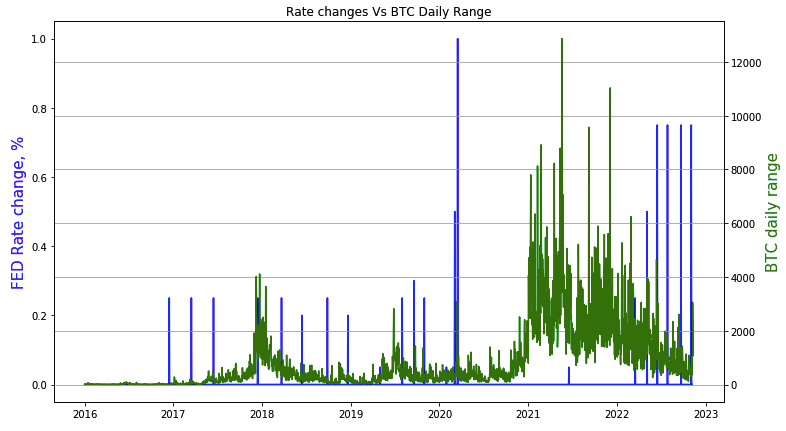
\includegraphics[width = \textwidth]{research_project/text/paper/range.png}
   \centering
   \caption{BTC volatility}
   \label{fig:range}
\end{figure}
The correlation between these two values was 0.012. So again, we could not find any significant relationship.
\newline
\section{Comments}
Our analysis was not exhaustive and could be improved in several ways. The methods used were quite rudimentary and given more time we would like to have considered other forms of analysis, most notably ARIMA and GARCH models.


In some pre-explanatory analysis, we did find large negative correlation over the past year. This can be seen in the figure below:
\begin{figure}[H]
   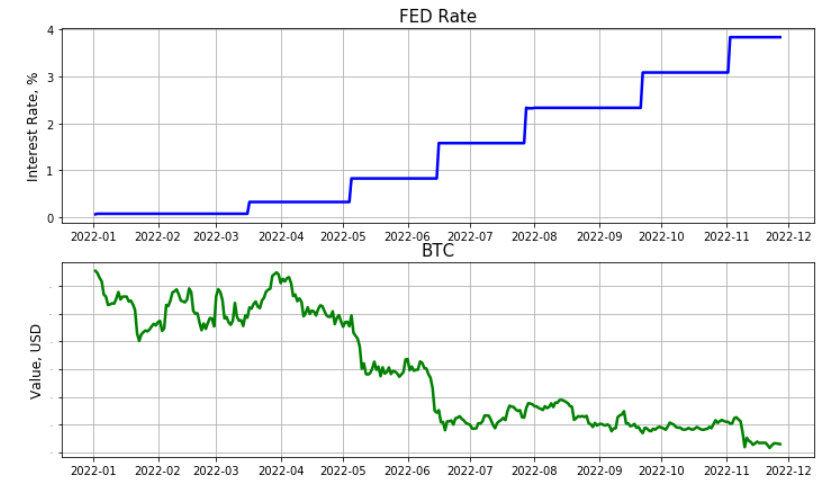
\includegraphics[scale=0.6]{research_project/text/paper/image2.png}
   \centering
   \caption{FED rate and BTC price over past year}
   \label{fig:comp_lastyear}
\end{figure}
\newline
Measuring the correlation here, we got a very strong negative value of -0.8914. This would most likely be the result of spurious correlation and not causation as the behaviour of the FED and most central banks has been to increases the interest rates quite rapidly to fight high inflation rates. Whether or not these decisions have been one of the drivers behind the decline in BTC can only be determined with time as we do not usually see such directional moves in a central banks monetary policy. 


\section{Conclusion}
In conclusion from all the analysis we have conducted we have no reason to believe the FED rate changes have any real effect of the BTC price movement in the short or long term, from all the analysis we see no significant evidence that there is any correlation in price movements and the change in the FED rate.
\newline
\newline
It is important to note that while there may not be a direct correlation between Federal Reserve interest rate changes and the price of Bitcoin, it is possible that macroeconomic factors influenced by Federal Reserve policies may have an indirect effect on the cryptocurrency market. For example, changes in the Federal Reserve's monetary policy can affect the value of traditional assets such as stocks and bonds, which in turn may affect investor behavior and their willingness to take on risk, including investing in cryptocurrency.
\newline
\newline
In conclusion, while it is possible that changes in the FED rate could influence the demand for Bitcoin, there are also a number of other factors that can impact the cryptocurrency's price. These include things like global economic conditions, investor sentiment, regulatory developments, and technological advances. As a result, it is difficult to draw a direct causal relationship between the FED rate and Bitcoin price.
\newline
\newline
This should be no surprise though, as one of the main functions of cryptocurrency is to act as a decentralized currency. If there were a significant relationship this would give power to the Federal Reserve and thus contradicting one of the fundamental principles behind cryptocurrencies. Most of these results can be examined in the application provided with this paper - we encourage the reader to play with the timeframe and also look at how other coins have behaved.


\end{document}
